\documentclass[11pt,oneside]{book}
\usepackage{amsmath}
\usepackage{amssymb}
\usepackage{amsthm}
\usepackage{amsfonts}
\usepackage{multirow}
\usepackage{float}
\usepackage{diagbox}
\usepackage{xcolor}
\usepackage{caption}
\usepackage{graphicx}
\graphicspath{{img/}}
\usepackage{paralist}
\usepackage{tikz}
\let\itemize\compactitem
\let\enditemize\endcompactitem
\let\enumerate\compactenum
\let\endenumerate\endcompactenum
\let\description\compactdesc
\let\enddescription\endcompactdesc
\setlength{\parindent}{0pt}
\title{Notes of Mathematical Analysis}
\author{}
\date{}
\newtheorem{theorem}{Theorem}[section]
\newtheorem*{lemma}{Lemma}
\newtheorem{definition}{Definition}[section]
\theoremstyle{definition}
\newtheorem{ex}{Exercise}[section]
\newtheorem*{answer}{Answer}
\newcommand\thmref[1]{\textbf{Theorem \ref{#1}}}
\newcommand\figref[1]{\textbf{Figure \ref{#1}}}
\begin{document}
\newtheorem*{tips}{\emph{TIPS}}
\chapter{Groups}
\section{Logical Symbols}
The logical symbols are a kind of symbols using for theoretical statements.
    \begin{table}[H]
        \centering
        \caption{Frequently-used Logical Symbols}
        \begin{tabular}{|c|c|}\hline
            Symbols&Meanings\\\hline
            $L\Longrightarrow P$& Proposition $L$ is contained in proposition $P$\\
            $L \Longleftrightarrow P $&Proposition $L$ is equivalent to proposition $P$\\
            $\lnot P$&Not $P$\\
            $L\wedge P$&Proposition $L$ and proposition $P$\\
            $L \vee P$&Proposition $L$ or proposition $P$\\
            \hline
        \end{tabular}
    \end{table}
e.g.\[((A\Longrightarrow B)\wedge(\lnot B)\Longrightarrow (\lnot A) )\]


stands for `` if $A$ is contained in  $B$,and $B$ is not true,then $A$ is not true''.

We also call $ A \Longleftrightarrow B$ ``$A$ is the necessary and suffiecent condition of $B$''.

The typical math proposition is like ``$A\Longrightarrow B$''.In order to prove this proposition ,we can use the  implication relationship \[A\Longrightarrow C_1\Longrightarrow \cdots \Longrightarrow C_n\Longrightarrow B\]The every implication relationship in this chain is general truth or proved proposition.

\begin{table}[H]
    \centering
    \caption{Truth Table}
    \begin{tabular}{|c|c|c|c|}
        \hline
        \multirow{2}{*}{$\lnot A$}                       & $A$                    & 0         & 1             \\ \cline{2-4} 
                                                 & $\lnot A$            & 1            & 0             \\ \hline
        \multirow{3}{*}{$A \vee B$}                       &       \diagbox{$A$}{$B$}     &    0        &       1        \\ \cline{2-4} 
                                                 &          0       &   0         &        1        \\ \cline{2-4} 
                                                 &       1         &  1        &        1       \\ \hline
        \multirow{3}{*}{$A \wedge B$}                       &        \diagbox{$A$}{$B$}    &           0&        1          \\ \cline{2-4} 
                                                 &     0         &     0          &      0          \\ \cline{2-4} 
                                                 &        1        &                0       &    1       \\ \hline
        \multirow{3}{*}{$A\Longrightarrow B$}                      &  \diagbox{$A$}{$B$} & 0  &  1 \\ \cline{2-4} 
                                                & 0  &  1 &  1 \\ \cline{2-4} 
                                                & 1  &  0 & 1  \\ \hline
        \end{tabular}
    \end{table}
\begin{question}$\lnot (A\wedge B )\Leftrightarrow (\lnot A \vee \lnot B)$.
\end{question}
\begin{proof}
    (Use the truth table)

    If $A$ is ture, $B$ is ture, $A\wedge B$ is ture. $\lnot (A\wedge B)$ is false.$\lnot A $ is false,$\lnot B$ is false, $(\lnot A \vee \lnot B)$ is false.

    If $A$ is ture, $B$ is false, $A\wedge B$ is false. $\lnot (A\wedge B)$ is true.$\lnot A $ is false,$\lnot B$ is true, $(\lnot A \vee \lnot B)$ is ture.

    If $A$ is flase, $B$ is true, $A\wedge B$ is false. $\lnot (A\wedge B)$ is true.$\lnot A $ is true,$\lnot B$ is false, $(\lnot A \vee \lnot B)$ is ture.

    If $A$ is false, $B$ is false, $A\wedge B$ is false. $\lnot (A\wedge B)$ is true.$\lnot A $ is true,$\lnot B$ is true, $(\lnot A \vee \lnot B)$ is ture.

    So
    \[\lnot (A\wedge B )\Leftrightarrow (\lnot A \vee \lnot B)\]
\end{proof}    

\begin{question}
    $(A \Rightarrow B)\Leftrightarrow\lnot A \vee B$.
\end{question}
\begin{proof}
    Firstly, we confirm the truth of \[(A \Rightarrow B)\Rightarrow\lnot A \vee B\]

    If $(A \Rightarrow B)$ is false, then $\lnot A \vee B$ is true.

    If $(A \Rightarrow B)$ is ture ,then we have two posibilities. The first is $A$ is ture, $B$ is true, so $\lnot A \vee B$ is true. The second is $A$ is false,then $B$ can be true or false, but $\lnot A \vee B$ will be true.

    Hence, $(A \Rightarrow B)\Rightarrow\lnot A \vee B$.

    Secondly, we prove \[(A \Rightarrow B)\Leftarrow\lnot A \vee B\]

    If $\lnot A \vee B$ is false, then $(A \Rightarrow B)$ is true.

    If $\lnot A \vee B$ is true, we have
    \begin{enumerate}
        \item $\lnot A$ is true, $B$ is false, then, $A$ is false, $(A \Rightarrow B)$ is true.
        \item $\lnot A$ is false, $B$ is true, then, $A$ is true, $(A \Rightarrow B)$ is true.
        \item $\lnot A$ is true, $B$ is true, then, $A$ is false, $(A \Rightarrow B)$ is true.
    \end{enumerate}

    So $(A \Rightarrow B)\Leftarrow\lnot A \vee B$.
\end{proof}



\section{Homomorphisms and subgroups}
\begin{ex}
    If $f: G \to H$ is a homomorphism of groups, then $f(e_G) = e_H$ and $f(a^{-1}) = f(a)^{-1}$ for all $a \in G$. Show by example that the first conclusion may be false if $G$, $H$ are monoids that are not groups.
\end{ex}

$$ $$

\begin{ex}
    A group $G$ is abelian if and only if the map $G\to G$ given by $x\to x^{-1}$ is automorphism.
\end{ex}

$$ $$

\begin{ex}
    Let $Q_8$ be the group(under ordinary matrix multiplication) generated by complex matrices $A = \begin{pmatrix}
        0 & 1 \\
        -1 & 0
    \end{pmatrix}$ and $B = \begin{pmatrix}
        0 & i\\
        i & 0
    \end{pmatrix}$, where $i^{2}=-1$. Show that $Q_8$ is a nonabelian group of order 8. $Q_8$ is called the quaternion group.
\end{ex}

$$ $$

\begin{ex}
    Let $H$ be the group(under ordinary matrix multiplication) of real matrices generated by $C = \begin{pmatrix}
        0 & 1\\
        -1 & 0
    \end{pmatrix}$ and $D = \begin{pmatrix}
        0 & 1\\
        1 & 0
    \end{pmatrix}$. Show that $H$ is a nonabelian group of order 8 which is not isomorphic to the quaternion group, but is isomorphic to the group $D_4^*$.
\end{ex}

$$ $$

\begin{ex}
    Let $S$ be a nonempty subset of a group $G$ and define a relation on $G$ by $a ~ b$ if and only if $ab^{-1}\in S$. Show that $~$ is an equivalence relation if and only if $S$ is a subgroup of $G$.
\end{ex}

$$ $$

\begin{ex}
    A nonempty finte subset of a group is s subgroup if and only if it is closed under the product in $G$.
\end{ex}

$$ $$

\begin{ex}
    If $n$ is a fixed integer, then $\{kn | n\in \mathbf{Z}\}\subset\mathbf{Z}$ is an additive subgroup of $\mathbf{Z}$, which is isomorphic to $\mathbf{Z}$. 
\end{ex}

$$ $$

\begin{ex}
    The set $\{\sigma\in S_n | \sigma(n) = n\}$ is a subgroup of $S_n$ which is isomorphic to $S_{n-1}$.
\end{ex}

$$ $$

\begin{ex}
    Let $f: G\to H$ be a homomorphism of groups, $A$ a subgroup of $G$, and $B$ a subgroup of $H$.
    \begin{enumerate}
        \item $\mathrm{Ker} f$ and $f^{-1}(B)$ are subgroups of $G$.
        \item $f(A)$ is a subgroup of $H$.
    \end{enumerate}
\end{ex}

$$ $$

\begin{ex}
    List all subgroups of $Z_2\oplus Z_2$. Is $Z_2\oplus Z_2$ isomorphic to $Z_4$?
\end{ex}

$$ $$

\begin{ex}
    If $G$ is a subgroup, then $C = \{a\in G| ax = xa \text{ for all } x\in G\}$ is a abelian subgroup of $G$. $C$ is called the center of $G$.
\end{ex}

$$ $$

\begin{ex}
    The group $D_4^*$ is not cyclic, but can be generated by two elements. The same is true of $S_n$(nontrivial). What is the minimal number of generators of the additive group $\mathbf{Z}\oplus\mathbf{Z}$?
\end{ex}

$$ $$

\begin{ex}
    If $G = \left\langle a \right\rangle $ is a cyclic group and $H$ is any group, then every homomorphism $f:G\to H$ is completely determined by the element $f(a)\in H$.
\end{ex}

$$ $$

\begin{ex}
    The following cyclic subgroups are all isomorphic: the multiplication group $\left\langle i \right\rangle$ in $\mathbf{C}$, the additive group $\mathbf{Z_4}$ and the subgroup $\left\langle \begin{pmatrix}
        1 & 2 & 3 & 4\\
        2 & 3 & 4 & 1
    \end{pmatrix}\right\rangle$ of $S_4$.
\end{ex}

$$ $$

\begin{ex}
    Let $G$ be a group and $\mathrm{Aut} G$ is the set of all automorphisms of $G$.
    \begin{enumerate}
        \item $\mathrm{Aut} G$ is a group with composition of functions as binary operation.
        \item $\mathrm{Aut} \mathbf{Z}\cong Z_2$ and $\mathrm{Aut} Z_6 \cong Z_2$; $\mathrm{Aut} Z_8\cong Z_2\oplus Z_2$; $\mathrm{Aut} Z_p\cong Z_{p-1}$ ($p$ prime).
        \item What is $\mathrm{Aut Z_n}$ for arbitrary $n\in \mathbf{N^*}$?
    \end{enumerate}
\end{ex}

$$ $$

\begin{ex}
    For each prime $p$ the additive subgroup $Z(p^\infty)$ of $\mathbf{Q}/\mathbf{Z}$ is generated by the set $\{\bar{1/p^n}|n\in \mathbf{N^*}\}$.
\end{ex}

$$ $$

\begin{ex}
    Let $G$ be an abelian group and let $H, K$ be subgroups of $G$. Show that the join $H\vee K$ is the set $\{ab|a\in H, b\in K\}$. Extend this result to any finite number of subgroups of $G$.
\end{ex}

$$ $$

\begin{ex}
    \begin{enumerate}
        \item Let $G$ be a group and $\{H_i| i\in I\}$ a family of subgroups. State and prove a condition that will imply that $\bigcup\limits_{i\in I}H_i$ is a subgroup, that is $\bigcup\limits_{i\in I}H_i = \left\langle\bigcup\limits_{i\in I}H_i\right\rangle$.
        \item Given an example of a group $G$ and a family of subgroups $\{H_i|i \in I\}$ such that $\bigcup\limits_{i\in I}H_i \neq \left\langle\bigcup\limits_{i\in I}H_i\right\rangle$.
    \end{enumerate}
\end{ex}

$$ $$

\begin{ex}
    \begin{enumerate}
        \item The set of all subgroups of a group $G$, partially ordered by set theoretic inclusion, forms a complete lattice in which the g.l.b of $\{H_i|i\in I\}$ is $\bigcap\limits_{i\in I}H_i$ and the l.u.b is $\left\langle\bigcap\limits_{i\in I}H_i\right\rangle$.
        \item Exhibit the lattice of subgroups of the groups $S_3, D_4^*, Z_6, Z_{27}$ and $Z_{36}$.
    \end{enumerate}
\end{ex}
\section{Cyclic groups}
\begin{ex}
    Let $a,b$ be elements of group $G$. Show that $\left| a \right| =\left| a^{-1} \right| $; $\left| ab \right| =\left| ba \right| $, and $\left| a \right| =\left| cac^{-1} \right| $ for all $c\in G$.
\end{ex}

\begin{answer}
    We only consider that $\left| a \right| , \left| b \right| , \left| c \right| $ are finite. Assume $a^{k}=e$, $(ab)^{m}=e$, $(ac^{-1})^{n}=e$, $kmn\neq 0$. $a^{k}\cdot(a^{-1})^{k}=e$, so $k$ sialso the order of $a^{-1}$, $\left| a^{-1} \right| =k$. $(ab)^{m}=e=a(ba)^{m-1}b\Rightarrow (ba)^{m-1}=a^{-1}b^{-1}$, $(ba)^{m}=a^{-1}b^{-1}ba=e$. $m$ is the order of $ba$. $(cac^{-1})^{r}=cac^{-1}cac^{-1}\cdots cac^{-1}=ca^{n}c^{-1}=e$, so $a^{n}=e$, whence $n=k$.
\end{answer}

$$ $$

\begin{ex}
    Let $G$ be an abelian group containing elements $a$ and $b$ of orders $m$ and $n$ respectively. Show that $G$ contains an element whose order is the least commom multiple of $m$ and $n$.
\end{ex}

\begin{answer}
    If $(m,n)=1$, we know that $\forall a^{i}, i=1,2,\dots, m$, $b^{j}, j=1, 2, \dots, n$, $a^{i}b^{j}\neq e$, since if $a^{i}=b^{j}$, $\left| a^{i} \right| =n=\left| b^{-j} \right| =\left| b^{j} \right| =m$. $G$ is abelian, so $(ab)^{k}=a^{k}b^{k}\Rightarrow \left| ab \right|=mn=\left[ m,n\right]$.

    If $m|n$ or $n|m$, then $a$ or $b$ is the element we want. We consider $m|\!\!/n$ and $n|\!\!/m$. Factorise $n=p_{1}^{t_{1}}p_{2}^{t_{2}}\cdots p_{l}^{t_{l}}$, $m=p_{1}^{s_{1}}p_{2}^{s_{2}}\cdots p_{l}^{s_{l}}$, where $p_{1},\cdots,p_{l}$ are primes and $t_{1},\cdots,t_{l}, s_{1},\cdots, s_{l}\geq 0$. We can choose a new arrangement of $p_{1},\cdots,p_{l}$ and make $t_{1}\geq s_{1}$, $t_{2}\geq s_{2}$,\dots, $t_{i}\geq s_{i}$, $t_{i+1}<s_{i+1}$,\dots, $t_{l}<s_{l}$.\[(m,n)=p_{1}^{s_{1}}\cdots p_{i}^{s_{i}}p_{i+1}^{t_{i+1}}\cdots p_{l}^{t_{l}}, \left[m,n\right]=p_{1}^{t_{1}}\cdots p_{i}^{t_{i}}p_{i+1}^{s_{i+1}}\cdots p_{l}^{s_{l}}\] Take $x=a^{{p_{i+1}^{s_{i+1}}}\cdots p_{l}^{s_{l}}}$, $y=b^{{p_{1}^{t_{1}}}\cdots p_{i}^{t_{i}}}$, then $\left| x \right| ={p_{1}^{t_{1}}}\cdots p_{i}^{t_{i}}$, $\left| y \right| =p_{i+1}^{s_{i+1}}\cdots p_{l}^{s_{l}}$. Thus $(x,y)=1$, the order of $xy$ is $\left| x \right| \cdot\left| y \right| =p_{1}^{t_{1}}\cdots p_{i}^{t_{i}}p_{i+1}^{s_{i+1}}\cdots p_{l}^{s_{l}}=\left[m,n\right]$.
\end{answer}

$$ $$

\begin{ex}
    Let $G$ be an abelian group of order $pq$, with $(p,q)=1$. Assume there exist $a,b\in G$ such that $\left| a \right| =p, \left| b \right| =q$ and show that $G$ is cyclic.
\end{ex}

\begin{answer}
    From \textbf{Exercise 1.3.2} we know $a^{i}b^{j}\neq e$ for $i<p$, $j<q$. $\left| G \right| =pq$ for all $a^{i}b^{j}$ and $a^{m}b^{n}$ with $i\neq m$, $b\neq n$, $a^{i}b^{j}\neq a^{m}b^{n}$. So $G$ can be generated by $ab$. $G$ is cyclic.
\end{answer}

$$ $$

\begin{ex}
    If $f:G\to H$ is a homomorphism, $a\in G$, and $f(a)$ has finte order in $H$, then $\left| a \right| $ is infinite or $\left| f(a) \right| $ divides $\left| a \right| $.
\end{ex}

\begin{answer}
    Assume $\left| f(a) \right| =n$, $\left| a \right| =m$, and $n|\!\!/m$. Trivially, $m\geq n$. Assume $\gcd(m,n)=k\leq n$. $a^{m}=e\Rightarrow f(a)^{m}=e'=f(a)^{n}$. By Bezout theorem $\exists x,y\in \mathbf{Z}$ s.t. $f(a)^{mx+ny}=f(a)^{k}=e'$, $k\leq n$, that's contradictory!
\end{answer}

$$ $$

\begin{ex}
    Let $G$ be the multiplicative group of all nonsingular $2\times 2$ matrices with rational entries. Show that $a=\begin{pmatrix}
        0 & -1\\1 & 0
    \end{pmatrix}$has order 4 and $b=\begin{pmatrix}
        0& 1\\-1&-1
    \end{pmatrix}$has order 3, but $ab$ has infinite order. Conversely, show that the additive group $Z_{2}\oplus \mathbf{Z}$ contains nonzero elements $a,b$ of infinite order such that $a+b$ has finite order. 
\end{ex}

\begin{answer}
    The verification of $\left| a \right| =4$ and $\left| b \right| =3$ is trivial. $ab=\begin{pmatrix}
        1 & 1\\ 0& 1
    \end{pmatrix}$ $\det(ab=\lambda I)=0\Rightarrow \lambda_{1}=\lambda_{2}=1$. $ab$ is not diagnizable. By induction, we have $(ab)^{n}=\begin{pmatrix}
        1 & 2^{n-1}\\ 0& 1
    \end{pmatrix}$ which means $(ab)$ has infinite order.

    For $a=(\bar{0},1), b=(\bar{0},-1)\in Z_{2}\oplus\mathbf{Z}$, $a,b$ have infinite order, but $a+b=(\bar{0},0)$ has finite order 1.
\end{answer}

$$ $$

\begin{ex}
    If $G$ is a cyclic group of order $n$ and $k| n$, then $G$ has exactly one subgroup of order $k$.
\end{ex}

\begin{answer}
    Assume $a^{n}=e$, $mk=n$, we verify that $\left\langle a^{m}\right\rangle$ is a subgroup of order $k$. $\forall x,y\in \mathbf{Z}_{+}$, $a^{xm}\cdot a^{-ym}=a^{(x-y)m}\in \left\langle a^{m}\right\rangle$, so $\left\langle a^{m}\right\rangle$ is a subgroup. $a^{km}=e$, $a^{sm}\neq e$ for $s<k$, so $\left| \left\langle a^{m}\right\rangle \right| =k$.
\end{answer}

$$ $$

\begin{ex}
    Let $p$ be prime and $H$ a subgroup of $Z(p^{\infty})$.
    \begin{enumerate}[(a)]
        \item Every element of $Z(p^{\infty})$ has finite order $p^{n}$ for some $n\geq 0$.
        \item If at least one element of $H$ has order $p^{k}$ and no element of $H$ has order greater than $p^{k}$, then $H$ is the cyclic subgroup generated by $\bar{1/p^{k}}$, whence $H\cong Z_{p^{k}}$.
        \item If there is no upper bound on the orders of elements of $H$, then $H=Z(p^{\infty})$.
        \item The only proper subgroups of $Z(p^{\infty})$ are the finite cyclic groups $C_{n}=\left\langle\bar{1/p^{n}}\right\rangle\,(n=1,2,\dots)$. Futhermore, $\left\langle0\right\rangle=C_{0}<C_{1}<C_{2}<C_{3}<\cdots$.
        \item Let $x_{1},x_{2},\dots$ be elements of an abelian group $G$ such that $\left| x_{1} \right| =p, px_{2}=x_{1},px_{3}=x_{2},\dots,px_{n+1}=x_{n},\dots$. The subgroup generated by the $x_{i}(i\geq 1)$ is isomorphic to $Z(p^{\infty})$. 
    \end{enumerate}
\end{ex}

\begin{answer}
    \begin{enumerate}[(a)]
        \item $\forall  x\in Z(p^{\infty})$, $x=\frac{a}{p^{n}}$ where $a<p^{n}$, $p|\!\!/a$. $p$ is a prime, so $\gcd(p,a)=1$. $m\cdot a|p^{n}\Rightarrow m=p^{n}$. Thus $m\cdot \frac{a}{p^{n}}=e$, $p^{n}$ is the smallest number satisfies it. $\frac{a}{p^{n}}$ has order $p^{n}$.
        \item For all $x\in Z(p^{\infty})$, if $x$ has order smaller than $p^{k}$, $x$ must have the form $x=\frac{a}{p^{i}}(i\leq k)$, $(p,a)=1$, so $x\in\left\langle\frac{1}{p^{k}}\right\rangle$. If not, assume $x=\frac{a}{p^{i}}(i>k)$, then $p^{k}\cdot x=\frac{a}{p^{i-k}}\neq 1$.
        \item Assume not, $H< Z(p^{\infty})$, $H\neq Z(p^{\infty})$. There exist $y\in H$ s.t. $y$ has order $p^{m}, m\geq n$. $y=\frac{b}{p^{m}}$, $(p,b)=1$, so there exists $b^{-1}\in\{1,2,\dots,p-1\}$, $bb^{-1}\equiv 1\mod p^{m}$. But $ab^{-1}p^{m-n}y=\frac{a}{p^{n}}=x\in H$, that's contradictory! Conversely, $H=Z(p^{\infty})$.
        \item From (b), we know that if there's least upper bound $p^{n}$ for elements in a subgroup $S$, then $S=C_{n}$.\[\left\langle0\right\rangle=C_{0}<C_{1}<C_{2}<C_{3}<\cdots<Z(p^{\infty})\] is easy to verify.
        \item We can verify that $f:x_{i}\mapsto \bar{\frac{1}{p^{i}}}$ is a well defined isomorphism. $f(e)=f(px_{1})=1$, $f(px_{i+1})=f(x_{i})=\frac{1}{p^{i}}=p\cdot \frac{1}{p^{i+1}}$. $f$ is obviously a bijection, so $H\cong Z(p^{\infty})$.
    \end{enumerate}
\end{answer}

$$ $$

\begin{ex}
    A group that has only a finite number of subgroups must be finite.
\end{ex}

\begin{answer}
    Suppose not. If the order of all subgroups are finite, $G$ must be finite. So there exists a infinite subgroup $H<G$. $\forall  a\in G$, if $\forall n\in \mathbf{N}$, $a^{n}\neq e$. then we can construct infinte subgroups $\left\langle a\right\rangle$, $\left\langle a^{2}\right\rangle$, $\left\langle a^{3}\right\rangle$\dots. If $\forall a\in G$, $\exists n\in \mathbf{N}$, $a^{n}=e$, so $\left\langle a\right\rangle$ is a proper subgroup of $G$, we can take $b\in G\backepsilon\left\langle a\right\rangle$ to construct another subgroup. By induction, there are infinte subgroups in $G$. That's contradictory, so $G$ must be finite.
\end{answer}

$$ $$

\begin{ex}
    If $G$ is an abelian group, then the set $T$ of all elements of $G$ with finite order is a subgroup of $G$.
\end{ex}

\begin{answer}
    We can easily verify that $\forall a,b\in S$, $\left| a \right| =m$, $\left| b \right| =n$ and $\left| ab^{-1} \right| \leq mn$ is finite. $T$ is a subgroup of $G$.
\end{answer}

$$ $$

\begin{ex}
    An infinite group is cyclic if and only if it is isomorphic to each of its proper subgroups.
\end{ex}

\begin{answer}
    If $G$ is cyclic, $G\cong \mathbf{Z}$, $S<G$. For any subgroup of $\mathbf{Z}$, it has the form $\{na\}, a\in \mathbf{Z}$. We can construct a isomorphism $f:n\mapsto na$, so $S\cong \{na\}\Rightarrow G\cong S$.

    If $\forall S<G$, $G\cong S$ and $\left| G \right| =\left| S \right| $ is finite. We prove there exists $S<G$ s.t. $\left| S \right| =\aleph_{0}$. Take $a\in G$ and $S=\{na|n\in \mathbf{Z}\}$, $S$ is a subgroup. If there exists $ma=0$, $S$ must be finite, contradictory! Thus, $S\cong \mathbf{Z}\cong G$. $G$ is a infinite cyclic group.
\end{answer}
\section{Cosets and counting}
\begin{ex}
    Let $G$ be a group and $\{H_{i}|i\in I\}$ a family of subgroups. Then for any $a\in G$, $(\bigcap\limits_{i}H_{i})a=\bigcap\limits_{i}H_{i}a$.
\end{ex}

$$ $$

\begin{ex}
    \begin{enumerate}[(a)]
        \item Let $H$ be the cyclic subgroup (of order 2) of $S_{3}$ generated by $\begin{pmatrix}
            1 & 2 &3\\2& 1&3
        \end{pmatrix}$. Then no left cosets of $H$ (except $H$ itself) is also a right coset. There exists $a\in S_{3}$ such that $aH\cap Ha=\{a\}$.
        \item If $K$ is the cyclic subgroup (of order 3) of $S_{3}$ generated by $\begin{pmatrix}
            1 & 2&3\\2& 3 &1
        \end{pmatrix}$, then every left coset of $K$ is also a right coset of $K$.
    \end{enumerate}
\end{ex}

$$ $$

\begin{ex}
    The following conditions on a finite group $G$ are equivalent.
    \begin{enumerate}[(i)]
        \item $\left| G \right| $ is prime.
        \item $G\neq \left\langle e\right\rangle$ and $G$ has no proper subgroups.
        \item $G\cong Z_{p}$ for some prime $p$.
    \end{enumerate}
\end{ex}

$$ $$

\begin{ex}
    Let $a$ be an integer and $p$ be a prime such that $p\nmid a$. Then $a^{p-1}\equiv 1\mod p$.
\end{ex}

$$ $$

\begin{ex}
    Prove that there are only two distinct groups of order 4 (up to isomorphism), namely $Z_{4}$ and $Z_{2}\oplus Z_{2}$.
\end{ex}

$$ $$

\begin{ex}
    Let $H,K$ be subgroups of a group $G$. Then $HK$ is a subgroup of $G$ if and only if $HK=KH$.
\end{ex}

$$ $$

\begin{ex}
    Let $G$ be a group of order $p^{k}m$, with $p$ prime and $(p,m)=1$. Let $H$ be a subgroup of order $p^{k}$ and $K$ a subgroup of order $p^{d}$, with $0<d\leq k$ and $K\not\subset H$. Show that $HK$ is not a subgroup of $G$.
\end{ex}

$$ $$

\begin{ex}
    If $H$ and $K$ are subgroups of finite index of a group $G$ such that $\left[G:H\right]$ and $\left[G:K\right]$ are relatively prime, then $G=HK$.
\end{ex}

$$ $$

\begin{ex}
    If $H,K$ and $N$ are subgroups of a group $G$ such that $H<N$, then $HK\cap N=H(K\cap N)$. 
\end{ex}

$$ $$

\begin{ex}
    Let $H,K,N$ be subgroups of a group $G$ such that $H<K$, $H\cap N=K\cap N$, and $HN=KN$. Show that $H=K$.
\end{ex}

$$ $$

\begin{ex}
    Let $G$ be a group of order $2n$; then $G$ contains an element of order 2. If $n$ is odd and $G$ abelian, there is only one element of order 2.
\end{ex}

$$ $$

\begin{ex}
    If $H$ and $K$ are subgroups of a group $G$, then $\left[H\vee K:H\right]\\\geq \left[K:H\cap K\right]$.
\end{ex}

$$ $$

\begin{ex}
    If $p>q$ are primes, a group of order $pq$ has at most one subgroup of order $p$.
\end{ex}

$$ $$

\begin{ex}
    Let $G$ be a group and $a,b\in G$ such that (i) $\left| a \right| =4=\left| b \right| $; (ii) $a^{2}=b^{2}$; (iii) $ba=a^{3}b=a^{-1}b$; (iv) $a\neq b$; (v) $G=\left\langle a,b\right\rangle$. Show that $\left| G \right| =8$ and $G\cong Q_{8}$.
\end{ex}
\section{Normality, quotient groups, and homomorphisms}
\begin{ex}
    If $N$ is a subgroup of index 2 in a group $G$, then $N$ is normal in $G$.
\end{ex}

\begin{answer}
    $\forall a\in G\backslash N$, $G=N\cup Na=N\cup aN$ and $N\cap Na=\varnothing$, $N\cap aN=\varnothing$. So $\forall x\in Na$, $x\in G\backslash N\Rightarrow x\in aN$, $Na\subset aN$. Similarly, $aN\subset Na$, whence $Na=aN$, $N\lhd G$.
\end{answer}

$$ $$

\begin{ex}
    If $\{N_{i}|i\in I\}$ is a family of normal subgroups of a group $G$, then $\bigcap\limits_{i\in I}N_{i}$ is a normal subgroup of $G$.
\end{ex}

\begin{answer}
    $\bigcap\limits_{i\in I}N_{i}$ is a subgroup of $G$. $N_{i} (i\in I)$ are normal subgroups of $G$, so $\forall a\in G$, $aN_{i}a^{-1}=\{an_{i}a^{-1}|n_{i}\in N_{i}\}=N_{i}$. $\forall x=ana^{-1}\in a(\bigcap\limits_{i\in I}N_{i})a^{-1}$, $n\in N_{i}\Rightarrow x\in a(\bigcap\limits_{i\in I}N_{i})a^{-1}\subset \bigcap\limits_{i\in I}aN_{i}a^{-1}=\bigcap\limits_{i\in I}N_{i}$. $\bigcap\limits_{i\in I}N_{i}$ are normal subgroup of $G$.
\end{answer}

$$ $$

\begin{ex}
    Let $N$ be a subgroup of a group $G$. $N$ is normal in $G$ if and only if (right) congruence modulo $N$ is a congruence relation on $G$.
\end{ex}

\begin{answer}
    If $N\lhd G$. $\forall a,b\in G$, $ab^{-1}\in N\Leftrightarrow a^{-1}b\in N$. If $a_{1}\equiv b_{1}\mod N$, $a_{2}\equiv b_{2}\mod N$, then $a_{2}b_{2}^{-1}\in N$, $a_{1}N=Na_{1}=Nb_{1}\Rightarrow a_{1}Nb_{1}^{-1}=N$. So $a_{1}a_{2}b_{1}^{-1}b_{2}^{-1}=(a_{1}a_{2})(b_{1}b_{2})^{-1}\in N$. Similarly, $(a_{1}a_{2})^{-1}(b_{1}b_{2})\in N$. Congruence modulo $N$ is a congruence relation.

    If congruence modulo $N$ is a congruence relation. $\forall a_{1}\equiv b_{1}\mod N$, $a_{2}\equiv b_{2}\mod N$, we will have $a_{1}a_{2}\equiv b_{1}b_{2}\mod N$. Take $n\in N$ and fix $a_{2}\in G$, define $b_{2}=n^{-1}a_{2}$. Then $\forall n\in N$, $n$ can be expressed as $a_{2}b_{2}^{-1}$, $a_{2}\equiv b_{2}\mod N$. $\forall a_{1}\in G$ and $\forall b_{1}\equiv a_{1}\mod N$, $a_{1}nb_{1}^{-1}=a_{1}a_{2}b_{2}^{-1}b_{1}^{-1}\in N$. Take $b_{1}=a_{1}$ and $n$ varies in $N$, $a_{1}na_{1}^{-1}\in N\Rightarrow a_{1}Na_{1}^{-1}\subset N$. Thus $N\lhd G$.
\end{answer}

$$ $$

\begin{ex}
    Let $\sim$ be an equivalence relation on a group $G$ and let $N=\{a\in G |a\sim e\}$. Then $\sim$ is a congruence relation on $G$ if and only if $N$ is a normal subgroup of $G$ and $\sim$ is congruence modulo $N$.
\end{ex}

\begin{answer}
    If $G\lhd N$ and $\sim$ is congruence modulo $N$. $\forall a\in G$, $aNa^{-1}\subset N$. $\forall a_{1}, b_{1}, a_{2}, b_{2}\in G$, $a_{1}b_{1}^{-1}\in N$, $a_{2}b_{2}^{-1}\in N$. $a_{1}a_{2}(b_{1}b_{2})^{-1}=a_{1}a_{2}b_{2}^{-1}b_{1}^{-1}$, denote $n=a_{2}b_{2}^{-1}\in N$, $a_{1}a_{2}b_{2}^{-1}b_{1}^{-1}=a_{1}nb_{1}^{-1}\in a_{1}Nb_{1}^{-1}$. $\forall n\in N$, there exists $n'=b_{1}^{-1}a_{1}, n'\in N$ s.t. $a_{1}n=b_{1}n'$. So $a_{1}nb_{1}^{-1}=b_{1}n'b_{1}^{-1}\in b_{1}Nb_{1}^{-1}\subset N$. That means $(a_{1}a_{2})(b_{1}b_{2})^{-1}\in N$, $a\sim b$ is a congruence relation.

    If $a\sim b$ is a congruence relation. We first prove $N$ is a subgroup of $G$. $\forall a\in N$, $a\sim e$, $a^{-1}\sim a^{-1}\Rightarrow e\sim a^{-1}$, so $a^{-1}\sim e$, $a^{-1}\in N$. $\forall a,b \in N$, $b^{-1}\sim e$, $a\sim e\Rightarrow ab^{-1}\in e$, thus $N<G$.

    $\forall x\in G$, $xN=\{xa|a\sim e\}=\{xa|xa\sim xe\}=\{ax|ax\sim e\}=Nx$, so $N$ is normal in $G$. $x\sim y\Leftrightarrow y\in xN$. $\sim$ is congruence modulo $N$.
\end{answer}

$$ $$

\begin{ex}
    Let $N<S_{4}$ consist of all those permutations $\sigma$ such that $\sigma(4)=4$. Is $N$ normal in $S_{4}$?
\end{ex}

\begin{answer}
    $N=\{(1),(12),(13),(23),(123),(132)\}$. Take $a=(14)\in G$, $a^{-1}=(14)$, $a^{-1}(12)a=(24)\notin N$. So $N$ is not normal in $S_{4}$.
\end{answer}

$$ $$

\begin{ex}
    Let $H<G$; then the set $aHa^{-1}$ is a subgroup for each $a\in G$, and $H\cong aHa^{-1}$. 
\end{ex}

\begin{answer}
    $H<G$, $aHa^{-1}=\{aha^{-1}|h\in H\}$. $\forall x,y\in aHa^{-1}$, $x=ah_{1}a^{-1}$, $y=ah_{2}a^{-1}$. $y^{-1}=ah_{2}^{-1}a^{-1}$, $xy=ah_{1}h_{2}^{-1}a^{-1}\in aHa^{-1}$, so $aHa^{-1}< G$.

     Take $f: H\to aHa^{-1}$ as $f(h)=aha^{-1}$. If $f(h_{1})=f(h_{2})=ah_{1}a^{-1}=ah_{2}a^{-1}$, then $h_{1}=h_{2}$, so $f$ is an injection. $f$ is a surjection because $\forall x\in aHa^{-1}$, $f(a^{-1}xa)=x$, $a^{-1}xa\in H$. In conclusion, $H\cong aHa^{-1}$.
\end{answer}

$$ $$

\begin{ex}
    Let $G$ be a finite group and $H$ a subgroup of $G$ of order $n$. If $H$ is the only subgroup of $G$ of order $n$, then $H$ is normal in $G$.
\end{ex}

\begin{answer}
    Applying \textbf{Exercise 1.5.6}, $\forall a\in G$, $aHa^{-1}\cong H$. $\left| aHa^{-1} \right| =\left| H \right| =n\Rightarrow aHa^{-1}=H$. Whence $H\lhd G$.
\end{answer}

$$ $$

\begin{ex}
    All subgroups of the quaternion group are normal.
\end{ex}

\begin{answer}
    $Q_{8}=\{a,b,a^{2},ba,ab,a^{2}b,ab^{2},a^{2}b^{2}\}$ where $a^{2}=b^{2}$, $a_{1}b=ba=a^{3}b$ and $\left| a \right| =\left| b \right| =4$. There are several subgroups $\{a,a^{2},ab^{2},a^{2}b^{2}\}$, $\{b, a^{2}, a^{2}b,\\ a^{2}b^{2}\}$, $\{ab,a^{2}b^{2}\}$, $\{ba,a^{2}b^{2}\}$, $\{a^{2},a^{2}b^{2}\}$. From \textbf{Exercise 1.5.1}, we know the first two subgroups are normal in $G$. For $\{ab,a^{2}b^{2}\}$, $\{ba,a^{2}b^{2}\}$, $\{a^{2},a^{2}b^{2}\}$, we can check that $ab, ba, a^{2}$ is commutative in $G$, that is $\forall x\in G$, $xabx^{-1}=ab$, $xbax^{-1}=ba$, $xa^{2}x^{-1}=a^{2}$. They are all normal in $G$.
\end{answer}

$$ $$

\begin{ex}
    \begin{enumerate}[(a)]
        \item If $G$ is a group, then the center of $G$ is a normal subgroup of $G$;
        \item the center of $S_{n}$ is the identity subgroup for all $n>2$.
    \end{enumerate}
\end{ex}

\begin{answer}
    \begin{enumerate}[(a)]
        \item By the definition of center $C$, $\forall x\in G$ and $a\in C$, $ax=xa$, so $xCx^{-1}=C$. $C$ is normal in $G$.
        \item $\forall x\in S_{n}$, $x$ can be expressed as \[x=(a_{1}a_{2}\cdots a_{i_{1}})(a_{i_{1}+1}a_{i_{1}+2}\cdots a_{i_{2}})\cdots(a_{i_{n-1}+1}a_{i_{n-1}+2}\cdots a_{i_{n}})\]
        Those cycles $(a_{1}a_{2}\cdots a_{i_{1}})$, $(a_{i_{1}+1}a_{i_{1}+2}\cdots a_{i_{2}})$, \dots, $(a_{i_{n-1}+1}a_{i_{n-1}+2}\cdots a_{i_{n}})$ are all disjoint, so they are commutative.

        If there exists cycles whose length is longer than 2. WLOG, assume $i_{1}>2$. Take $y=(a_{1}a_{2})$, \[y^{-1}xy=(a_{1}a_{2})(a_{1}a_{2}\cdots a_{i_{1}})(a_{1}a_{2})\cdots(a_{i_{n-1}+1}a_{i_{n-1}+2}\cdots a_{i_{n}})\] $(a_{1}a_{2})(a_{1}a_{2}\cdots a_{i_{i}})(a_{1}a_{2})=(a_{2}a_{1}a_{3}\cdots a_{i_{1}})$, so $y^{-1}xy\neq x$, $x\notin C$. 

        If $x=(a_{1}a_{2})(a_{3}a_{4})\cdots(a_{2n-1}a_{2n})$ and $n\geq 2$. Take $y=(a_{1}a_{3})$, \[\begin{aligned}
            y^{-1}xy&=(a_{1}a_{3})(a_{1}a_{2})(a_{3}a_{4})\cdots(a_{2n-1}a_{2n})(a_{1}a_{3})\\&=(a_{1}a_{3})(a_{1}a_{2})(a_{3}a_{4})(a_{1}a_{3})\cdots(a_{2n-1}a_{2n})\\&=(a_{1}a_{4})(a_{2}a_{3})\cdots(a_{2n-1}a_{2n})\\&\neq x
        \end{aligned}\] So $x\notin C$.

        If $x=(a_{1}a_{2})$. Take $y=(a_{1}a_{3})$, $y^{-1}xy=(a_{2}a_{3})\neq x$, so $x\notin C$.

        In conclusion, $C=\{(1)\}$.
    \end{enumerate}
\end{answer}

$$ $$

\begin{ex}
    Find subgroups $H$ and $K$ of $D_{4}^{*}$ such that $H\lhd K$ and $K\lhd D_{4}^{*}$, but $H$ is not normal in $D_{4}^{*}$.
\end{ex}

\begin{answer}
    $D_{4}^{*}=\{I,R,R^{2},R^{3},T_{x},T_{y},T_{13},T_{24}\}$. Take $K=\{I, R, T_{x}, T_{y}\}$, $H=\{I, T_{x}\}$. We can easily verify that $H\lhd K$ and $K\lhd  D_{4}^{*}$ but $K\ntriangleleft  D_{4}^{*}$.
\end{answer}

$$ $$

\begin{ex}
    If $H$ is a cyclic subgroup of a group $G$ and $H$ is normal in $G$, then every subgroup of $H$ is normal in $G$.
\end{ex}

\begin{answer}
    Assume $K<H\lhd G$, $H$ has the generator $a$, and $K$ has the generator $a^{n}$. Here we used: \emph{Every subgroup of a cyclic group is cyclic.} This can be easily proved by the conclusion $H\cong Z_{m}$ for some $m\in \mathbf{Z}$. $\forall x\in G$, $h=a^{s}\in H$, $x^{-1}a^{s}x=a^{t}\in H$. Assume $x^{-1}ax=a^{m}$, then $x^{-1}a^{n}x=(x^{-1}ax)^{n}=a^{mn}=a^{k}$, so $n|k$, $a^{k}\in K$. $x^{-1}Kx\subset K$, $K$ is normal in $G$.
\end{answer}

$$ $$

\begin{ex}
    If $H$ is a normal subgroup of a group $G$ such that $H$ and $G/H$ are finitely generated, then so is $G$.
\end{ex}

\begin{answer}
    Assume $A=\{a_{1},a_{2},\dots, a_{m}\}$, $B=\{b_{1}, b_{2},\dots, b_{n}\}$. $H=\left\langle A\right\rangle$, $G /H=\left\langle \{Hb_{i}|b_{i}\in B\}\right\rangle$. We prove that $G$ can be generated by $A\cup B$. $\forall x\in G$, $x$ is in one of the right cosets of $H$, $x\in Ha$. $Ha\in G /H$ so $Ha=\prod\limits_{b_{i}\in B}Hb_{i}^{s_{i}}=H(\prod\limits_{b_{i}\in B}b_{i}^{s_{i}})$. Thus $a^{-1}(\prod\limits_{b_{i}\in B}b_{i}^{s_{i}})=a'\in H$. $H$ is generated by $A$ so $xa^{-1}=\prod\limits_{a_{i}\in A}a_{i}^{t_{i}}$, $a'=\prod\limits_{a_{i}\in A}a_{i}^{-r_{i}}$. Then \[x=(\prod\limits_{a_{i}\in A}a_{i}^{t_{i}+r_{i}})(\prod\limits_{b_{i}\in B}b_{i}^{s_{i}})\in\left\langle A\cup B\right\rangle\] Thus $G\subset\left\langle A\cup B\right\rangle$ is finitely generated.
\end{answer}

$$ $$

\begin{ex}
    \begin{enumerate}[(a)]
        \item Let $H\lhd G$, $K\lhd G$. Show that $H\vee K$ is normal in $G$.
        \item Prove that the set of all normal subgroups of $G$ forms a complete lattice under inclusion.
    \end{enumerate}
\end{ex}

\begin{answer}
    \begin{enumerate}[(a)]
        \item $\forall x\in G$, $a\in H\vee K$, we need to prove $x^{-1}ax\in H\vee K$. $a\in H\vee K$ so $a$ can be expressed  as \[a=b_{1}^{n_{1}}b_{2}^{n_{2}}\cdots b_{t}^{n_{t}}\quad \text{where } b_{i}\in H \text{ or } b_{i}\in K, i=1,2,\dots,t\] so $x^{-1}ax= x^{-1}b_{1}^{n_{1}}\cdots b_{t}^{n_{t}}x =(x^{-1}b_{1}x)^{n_{1}}(x^{-1}b_{2}x)^{n_{2}}\cdots (x^{-1}b_{t}x)^{n_{t}}$.\\ $H\lhd G$, $K\lhd G$, so $x^{-1}b_{i}x\in H\vee K, i=1,2,\dots,t$ and \[x^{-1}ax=(x^{-1}b_{1}x)^{n_{1}}(x^{-1}b_{2}x)^{n_{2}}\cdots (x^{-1}b_{t}x)^{n_{t}}\in H\vee K\] $H\vee K\lhd G$.
        \item Actually, in \textbf{Exercise 1.2.19} and (a), we have proved lub exists.
        
        Now we only consider glb. For $H\lhd G$, $K\lhd G$. If $H\cap K\lhd G$, then their glb is $H\cap K$. If not, assume there exists $A<H\cap K$, $B<H\cap K$, $A$, $B$ are both normal in $H$ and $K$. And there doesn't exists $I$ s.t. $A\lhd I\lhd H$, $A\lhd I\lhd K$, $B\lhd I\lhd H$, $B\lhd I\lhd K$. Just like the figure:
        
        \begin{figure}[H]\centering
            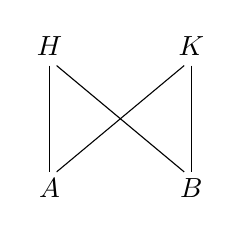
\begin{tikzpicture}[scale=0.9]
                \node [above] at (0,0) {$A$};
                \node [above] at (0,2) {$H$};
                \node [above] at (2,2) {$K$};
                \node [above] at (2,0) {$B$};
                \draw [-] (1.9,2) to (0.1,0.5);
                \draw [-] (2,2) to (2,0.5);
                \draw [-] (0,2) to (0,0.5);
                \draw [-] (0.1,2) to (1.9,0.5);
            \end{tikzpicture}
        \end{figure}
        But $A<H\cap K$, $B<H\cap K\Rightarrow A\vee B<H\cap K$. So $A\vee B\lhd H$, $A\vee B\lhd K$. That's contradictory! There is only one lower bound for $\{H,K\}$. Notice that $\{e\}<H\cap K$ so there exists at least one subgroup satisfies the condition. We have proved normality forms a lattice.
    \end{enumerate}
\end{answer}

$$ $$

\begin{ex}
    If $N_{1}\lhd G_{1}$, $N_{2}\lhd G_{2}$ then $(N_{1}\times N_{2})\lhd (G_{1}\times G_{2})$ and $(G_{1}\times G_{2})/(N_{1}\times N_{2})\cong (G_{1}/N_{1})\times(G_{2}/N_{2})$.
\end{ex}

\begin{answer}
    Take $a\in (N_{1}\times N_{2})$, $a=(n_{1},n_{2})$ where $n_{1}\in N_{1}$, $n_{2}\in N_{2}$. $\forall x\in (G_{1}\times G_{2})$, $x=(g_{1},g_{2})$ where $g_{1}\in G_{1}$, $g_{2}\in G_{2}$. $x^{-1}=(g_{1}^{-1},g_{2}^{-1})$, $x^{-1}ax=(g_{1}^{-1}n_{1}g_{1},g_{2}^{-1}n_{2}g_{2})$. $N_{1}\lhd G_{1}$, $N_{2}\lhd G_{2}$, so $g_{1}^{-1}n_{1}g_{1}\in N_{1}$, $g_{2}^{-1}n_{2}g_{2}\in N_{2}$. $x^{-1}ax\in (N_{1}\times N_{2})$. Thus $(N_{1}\times N_{2})\lhd (G_{1}\times G_{2})$.

    Assume $G_{1}=\bigcup\limits_{i\in I}N_{1}a_{i}$, $G_{2}=\bigcup\limits_{j\in J}N_{2}b_{j}$. Then $G_{1}\times G_{2}=\bigcup\limits_{i\in I}N_{1}a_{i}\times \bigcup\limits_{j\in J}N_{2}b_{j}$. Denote $A=\{a_{i}|i\in I\}$, $B=\{b_{j}|j\in J\}$. We construct two bijections $(G_{1}\times G_{2})/(N_{1}\times N_{2})\to A\times B$ and $(G_{1}/N_{1})\times(G_{2}/N_{2})$.\[f: N_{1}a_{i}\times N_{2}b_{j}\mapsto (a_{i},b_{j})\]\[g: (N_{1}a_{i}, N_{2}b_{j})\mapsto (a_{i},b_{j})\] Take $h=g^{-1}\circ f$, $f,g$ are bijections, so $h$ is an isomorphism. $(G_{1}\times G_{2})/(N_{1}\times N_{2})\cong (G_{1}/N_{1})\times(G_{2}/N_{2})$.
\end{answer}

$$ $$

\begin{ex}
    Let $N\lhd G$ and $K\lhd G$. If $N\cap K=\left\langle e\right\rangle$ and $N\vee K=G$, then $G/N\cong K$.
\end{ex}

\begin{answer}
    Assume $G=\bigcup\limits_{i\in I}Na_{i}$, we construct $f:k \to G /N$. We prove that $\forall x,y\in K$, $x,y$ belong to different cosets of $N$. Suppose not. $\exists x,y \in K$, $x,y\in Na_{i}$, then $xy^{-1}\in N\Rightarrow x=y$. That's contradictory! So $f$ is a monomorphism.

    $G=H\vee K$, so $G=HK$. we can write $x$ as $pq$, where $p\in H$, $q\in K$. $\left| G/H \right|=\left[G:H\right]=\left[HK:H\right]=\left[K:K\cap H\right]=\left| K \right| $. $f$ is a epimorphism.
    
    Thus, $G /N\cong K$.
\end{answer}

$$ $$

\begin{ex}
    If $f:G\to H$ is a homomorphism, $H$ is abelian and $N$ is a subgroup of $G$ containing $\mathrm{Ker}f$, then $N$ is normal in $G$.
\end{ex}

\begin{answer}
    Assume there exists $x\in G$, $x\notin N$ s.t. $f(x)\in f(N)$. $\exists n\in N$, $f(x)=f(n)$, $f(xn^{-1})=f(x)f(n)^{-1}=e'\Rightarrow xn^{-1}\in\mathrm{Ker}f\Rightarrow x\in N$. That's contradictory! $\forall x\in G$, $n\in N$, $f(x^{-1}nx)=f(x^{-1})f(n)f(x)=f(n)\in f(N)$, so $x^{-1}nx\in N$. Thus, $N\lhd G$.
\end{answer}

$$ $$

\begin{ex}
    \begin{enumerate}[(a)]
        \item Consider the subgroups $\left\langle 6\right\rangle$ and $\left\langle 30\right\rangle$ of $\mathbf{Z}$ and show that $\left\langle 6\right\rangle /\left\langle 30\right\rangle\cong Z_{5}$.
        \item For any $k,m>0$, $\left\langle k\right\rangle /\left\langle km\right\rangle\cong Z_{m}$; in particular, $\mathbf{Z}/\left\langle m\right\rangle=\left\langle 1\right\rangle /\left\langle m\right\rangle\cong Z_{m}$.
    \end{enumerate}
\end{ex}

\begin{answer}
    \begin{enumerate}[(a)]
        \item $\left\langle 6\right\rangle=\{6n|n\in \mathbf{Z}\}$, $\left\langle 30\right\rangle=\{30n|n\in \mathbf{Z}\}$. So $\left\langle 6\right\rangle/\left\langle 30\right\rangle=\{\left\langle 30\right\rangle, \left\langle 30\right\rangle +6, \left\langle 30\right\rangle +12, \left\langle 30\right\rangle +18, \left\langle 30\right\rangle +24\}\cong Z_{5}$
        \item $\left\langle km\right\rangle\lhd \left\langle k\right\rangle$, $\left\langle k\right\rangle=\bigcup\limits_{i\in I}(\left\langle km\right\rangle +a_{i})$. For $x\in \left\langle k\right\rangle$, $x\equiv a_{i}\mod km$, then $x\in \left\langle km \right\rangle +a_{i}$. $f:\left\langle k\right\rangle/\left\langle km\right\rangle\to \{a_{i}|i\in I\}$ defined by $f(\left\langle km\right\rangle +a_{i})=a_{i}$ is a bijection. We check that $g: \{a_{i}|i\in I\}\to Z_{m}$ is also a bijection. Define $b_{i}\equiv \frac{a_{i}}{k}\mod m$, $g(a_{i})=b_{i}$. If there exists $b_{i}=b_{j}$ for $i\neq j$, $a_{i}\equiv a_{j}\mod km$. That's contradictory! So $g$ is an injection. $g$ is obviously a surjection, so $g$ is a bijection. Take $h= g\circ f:\left\langle k\right\rangle /\left\langle km \right\rangle\to Z_{m}$ is a isomorphism, so $\left\langle k\right\rangle /\left\langle km \right\rangle\cong Z_{m}$.
    \end{enumerate}
\end{answer}

$$ $$

\begin{ex}
    If $f: G \to H$ is a homomorphism with kernel $N$ and $K<G$, then prove that $f^{-1}(f(K))=KN$. Hence $f^{-1}(f(K))=K$ if and only if $N<K$.
\end{ex}

\begin{answer}
    Take $x\in f^{-1}(f(K))$, then there exists $k\in K$ s.t. $f(x)=f(k)$. $f(xk^{-1})=f(x)f(k)^{-1}=e'\in f(K) \Rightarrow xk^{-1}\in\mathrm{Ker}f=N$. Thus, $x\in Nk\subset NK$, $f^{-1}(f(K))\subset NK$.

    $\forall x=nk\in NK$, where $n\in N$ and $k\in K$. $f(x)=f(n)f(k)=e'f(k)\in f(K)$, so $NK\subset f^{-1}(f(K))$.

    Thus, $f^{-1}(f(K))=NK$. Hence $f^{-1}(f(K))=K$ if and only if $N<K$.
\end{answer}

$$ $$

\begin{ex}
    If $N\lhd G$, $\left[G:H\right]$ finite, $H<G$, $\left| H \right| $ finite, and $\left[G:N\right]$ and $\left| H \right| $ are relatively prime, then $H<N$.
\end{ex}

\begin{answer}
    $N\lhd G\Rightarrow NH<G$. By the second isomorphism theorem, $NH /N\cong H/H\cap N\Rightarrow \left[NH:N\right]=\left[H:H\cap N\right]$. Assume $\left[G:N\right]=m$, $\left| H \right| =n$, $\left| G \right| =mnp$ where $(m,n)=1$. Then $\left| N \right| =np$, $N<NH$, assume $\left| NH \right| =knp$, $NH<G\Rightarrow knp|mnp\Rightarrow k|m$. $\left[NH:N\right]=\left[H:H\cap N\right]=k\Rightarrow k|n$. So $k=1$, $NH=N$ which means $H<N$.
\end{answer}

$$ $$

\begin{ex}
    If $N\lhd G$, $\left| N \right|$ finite, $H<G$, $\left[G:N\right] $ finite, and $\left[G:H\right]$ and $\left| N \right| $ are relatively prime, then $N<H$.
\end{ex}

\begin{answer}
    $N\lhd G\Rightarrow NH<G$. By the second isomorphism theorem, $NH /N\cong H/H\cap N\Rightarrow \left[NH:N\right]=\left[H:H\cap N\right]$. Assume $\left[G:H\right]=m$, $\left| N \right| =n$, $\left| G \right| =mnp$ where $(m,n)=1$. Then $\left| H \right| =np$, $H<NH$, assume $\left| NH \right| =knp$, $NH<G\Rightarrow knp|mnp\Rightarrow k|m$. $\left[NH:N\right]=\left[H:H\cap N\right]=kp\Rightarrow kp|np\Rightarrow k|n$. So $k=1$, $NH=H$ which means $N<H$.
\end{answer}

$$ $$

\begin{ex}
    If $H$ is a subgroup of $Z(p^{\infty})$ and $H\neq Z(p^{\infty})$, then $Z(p^{\infty}) /H\cong Z(p^{\infty})$.
\end{ex}

\begin{answer}
    From \textbf{Exercise 1.3.7}(b), we know that $H$ has the form $\left\langle \bar{\frac{1}{p^{n}}}\right\rangle$. Take $x_{i}=\bar{\frac{1}{p^{n+i}}}+H$, $x_{1}=\bar{\frac{1}{p^{n+1}}}+H$. \[\sum_{m=1}^{p}x_{1}=\bar{\frac{p}{p^{n+1}}}+pH=\bar{\frac{1}{p^{n}}}+H=H\] \[\sum_{m=1}^{p}x_{i}=\bar{\frac{p}{p^{n+i}}}+pH=\bar{\frac{1}{p^{n+i-1}}}+H=x_{i-1}\] Take $A=\{x_{i}|i\in \mathbf{Z}_{+}\}$, $\left\langle A\right\rangle\cong Z(p^{\infty})$ by \textbf{Exercise 1.3.7}(e). $\forall x\in \left\langle A\right\rangle$, $x\in Z(p^{\infty}) /H$, so $\left\langle A\right\rangle\subset Z(p^{\infty}) /H$. Take $x\in Z(p^{\infty}) /H$, $x=y+H$ where $y=\sum\limits_{i=1}^{m}\frac{a_{i}}{p^{n+i}}$, $x=\sum\limits_{i=1}^{m}(\frac{a_{i}}{p^{n+i}}+H)\in \left\langle A\right\rangle$. Thus, $Z(p^{\infty}) /H\subset \left\langle A\right\rangle$, $\left\langle A\right\rangle=Z(p^{\infty}) /H\cong Z(p^{\infty})$.
\end{answer}
\end{document}